\documentclass[
	german,% Main language as global option
	accentcolor=9c,% Choose accent color: For a list of available colors see the full tudapub documentation
	accept-missing-logos=true,% No error in case logo files are not available
%	logofile=example-image,% In case logo should be replaced
]{tudabeamer}
\usepackage{tikz}
\usetikzlibrary{arrows.meta,positioning,shapes.geometric}
\usepackage[ngerman]{babel}
\usepackage[autostyle]{csquotes}
\usepackage{natbib}   % reference
\usepackage{booktabs} % table
\usepackage{multirow} % table
\usepackage{pgfplots}
\usepackage{algorithm}
\usepackage{algpseudocode}


% MACROS
\renewcommand{\v}{\TextOrMath{\textv}{\mathbf{v}}}
\newcommand{\g}{\mathbf{g}}
\newcommand{\x}{\mathbf{x}}
\newcommand{\y}{\mathbf{y}}
\renewcommand{\u}{\TextOrMath{\textu}{\mathbf{u}}}
\renewcommand{\k}{\mathbf{k}}

\renewcommand{\b}{\mathbf{b}}
\newcommand{\n}{\mathbf{n}}
\newcommand{\normal}{\boldsymbol{n}} 

\newcommand{\h}{\boldsymbol{h}} 
\newcommand{\nsigma}{\boldsymbol{n}_\Sigma} 
\newcommand{\vel}{\boldsymbol{v}} 
\newcommand{\fsigma}{\boldsymbol{f}_\Sigma} 
\newcommand{\frad}{\boldsymbol{f}_{rad}} 
\newcommand{\hatp}{\hat{p}}
\newcommand{\hatpre}{\hat{p}_{re}}
\newcommand{\hatpim}{\hat{p}_{im}}
\newcommand{\tn}{t^n}
\newcommand{\tnn}{t^{n+1}}
\newcommand{\Sf}{\mathbf{S}_f}

\pgfplotsset{compat=1.18}


\setbeamerfont{frametitle}{size=\large}
\addtobeamertemplate{frametitle}{\vspace{-1em}}{}


\newcommand*{\code}[1]{\texttt{#1}}
\newcommand*{\placeholderfig}[2]{%
    \fbox{\begin{minipage}[c][#2][c]{#1}\centering\small Platzhalter: Bild einfuegen\end{minipage}}%
}
\title{NUMERICAL STUDY OF ACOUSTIC LEVITATION}
\author{Chuanchao Xu}
\department{Mathematics}
\institute{Mathematical Modeling and Analysis}
\date{\today}% In case \today should not be used

\begin{document}
\maketitle
%\tableofcontents

\section{090626}
\begin{frame}{Ablauf des heutigen Treffens}
    \begin{enumerate}
        \item \textbf{Kurzer Fortschrittsbericht seit dem letzten Treffen}
        \begin{itemize}
            \item Axisymmetrisches, lokal verfeinertes Mesh mit cfMesh:
            Gor'kov-Verifikation und Gleichgewichtssuche werden möglich.
            \item Tensorielle PML: kleinere Dämpfungskoeffizienten und ein
            geringeres Risiko numerischer Reflexionen.
        \end{itemize}
        \item \textbf{Gemeinsame Durchsicht des Papers}
        \begin{itemize}
            \item Struktur, Ergebnisse und noch offene Punkte.
        \end{itemize}
        \item \textbf{Diskussion des Experimentplans}
        \begin{itemize}
            \item Zielgrößen, Parameterbereich und Vergleich mit den Simulationen.
        \end{itemize}
    \end{enumerate}
\end{frame}


\begin{frame}{Axisymmetrisches, lokal verfeinertes Mesh}
    \begin{columns}
    \column{.52\linewidth}
    \begin{itemize}
        \item cfMesh erzeugt zunächst ein zweidimensionales, lokal verfeinertes Mesh.
        \item \code{extrudeMesh} überführt dieses in eine axisymmetrische
        $1^\circ$-Wedge-Domäne.
        \item Automatisierter Workflow:
        \begin{enumerate}
            \item \code{prepareCase}
            \item \code{cartesian2DMesh}
            \item \code{extrudeMesh} als $1^\circ$-Wedge
            \item \code{postMesh}
        \end{enumerate}
        \item Lokale Verfeinerung und Body-Fit nahe \code{dropWall};
        gröbere Zellen im entfernten Bereich.
    \end{itemize}
    \column{.48\linewidth}
    \begin{center}
        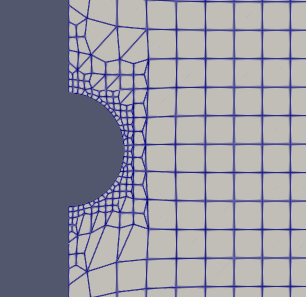
\includegraphics[height=3.2cm]{figures/meshLocalRefine.png}

        \vspace{0.2cm}
        \scriptsize Axisymmetrisches Wedge-Mesh mit lokaler Verfeinerung nahe \code{dropWall}.
    \end{center}
    \end{columns}
\end{frame}

\begin{frame}{Das Mesh ermöglicht die Gor'kov-Verifikation}
    \begin{columns}
    \column{.54\linewidth}
    \begin{itemize}
        \item Kleine Kugeln können als lokal verfeinerte, feste
        \code{dropWall}-Geometrie aufgelöst werden.
        \item Zwei komplementäre Frequenzdomänenpfade:
        \begin{enumerate}
            \item Gor'kov-Kraft aus dem ungestörten akustischen Feld,
            \item direkte Kraft aus der Druckintegration auf \code{dropWall}.
        \end{enumerate}
        \[
            U_G = V_p\left(f_1 E_p-\frac{3}{2}f_2 E_k\right),
            \qquad
            \mathbf{F}_G=-\nabla U_G .
        \]
        \item Ergebnis: gute Übereinstimmung für kleine Partikel;
        mit wachsendem Radius verliert die Punktpartikel-Näherung ihre Gültigkeit.
    \end{itemize}
    \column{.46\linewidth}
    \begin{center}
        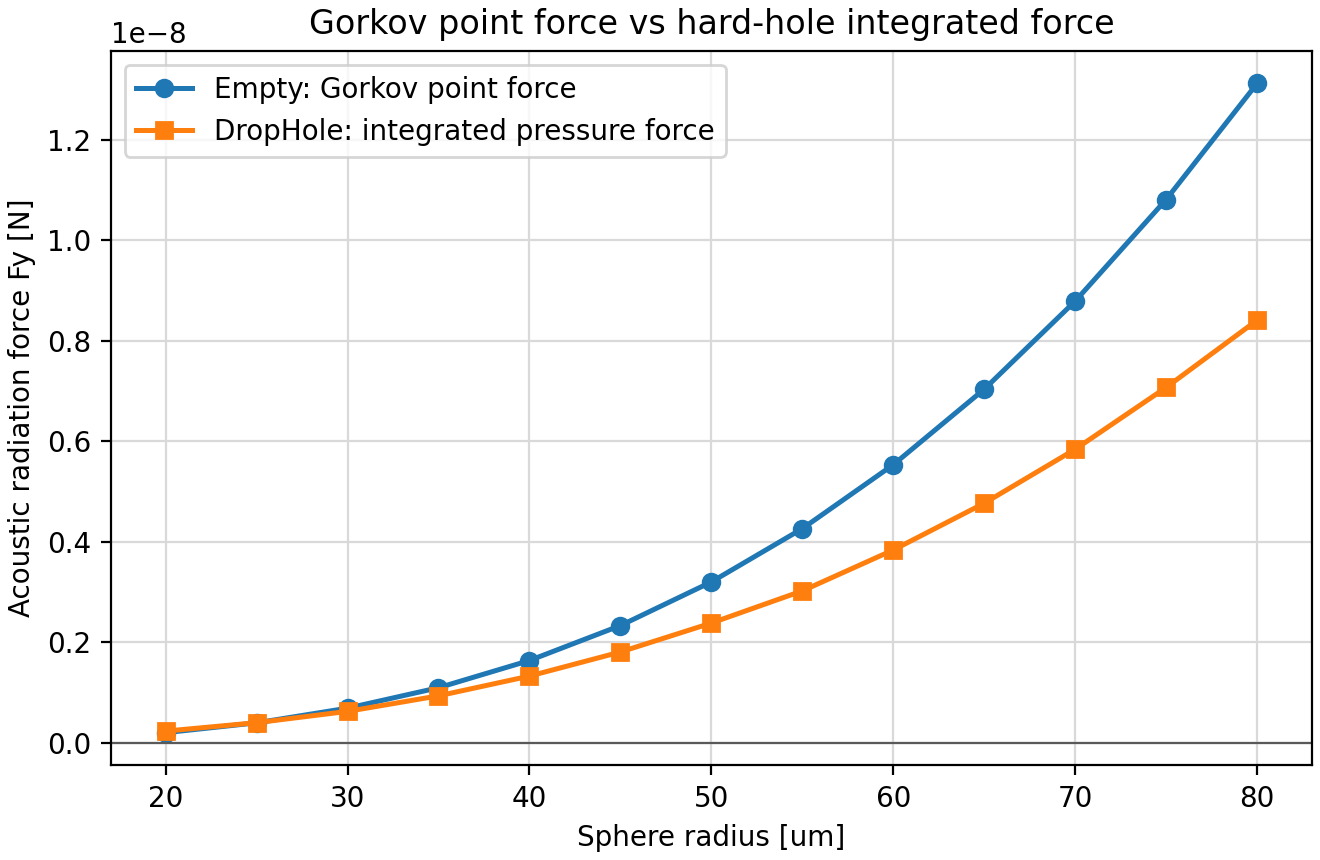
\includegraphics[width=\linewidth]{figures/gorkovVsHoleForce.png}

        \vspace{0.2cm}
        \scriptsize Vergleich zwischen Gor'kov-Punktkraft und integrierter \code{dropWall}-Kraft.
    \end{center}
    \end{columns}
\end{frame}

\begin{frame}{Das Mesh ermöglicht die Gleichgewichtssuche}
    \begin{columns}
    \column{.55\linewidth}
    \begin{itemize}
        \item Solver: \code{acousticDropEquilibriumFoam}.
        \item Das Body-Fit-Mesh erlaubt die iterative Änderung von Position und
        Form der festen Tropfenoberfläche.
        \item Iterativer Ablauf:
        \begin{enumerate}
            \item Akustisches Feld für feste Tropfenform lösen.
            \item Kraft auf \code{dropWall} integrieren.
            \item Vertikale Position bis $F_y \approx \rho_l V g$ korrigieren.
            \item Formresiduum aus
            \[
                p_r+\rho_l g y+\gamma\kappa = h
            \]
            auswerten.
            \item Normalen-Update mit Volumenkorrektur, dann wiederholen.
        \end{enumerate}
    \end{itemize}
    \column{.45\linewidth}
    \begin{center}
        \begin{tikzpicture}[
            scale=0.9,
            transform shape,
            >=Stealth,
            node distance=0.24cm,
            every node/.style={font=\scriptsize, align=center},
            flowstep/.style={draw, rounded corners=1.5pt, minimum width=3.35cm, minimum height=0.43cm, fill=TUDa-9c!8},
            test/.style={draw, diamond, aspect=2.45, inner sep=0.6pt, text width=1.75cm, fill=TUDa-9c!18},
            update/.style={draw, rounded corners=1.5pt, minimum width=1.05cm, minimum height=0.43cm, fill=TUDa-9c!14},
            arrow/.style={->, line width=0.35pt},
            loop/.style={->, line width=0.35pt, rounded corners=3pt}
        ]
            \node[flowstep] (shape) {aktuelle Tropfenform};
            \node[flowstep, below=of shape] (solve) {Helmholtz-Feld loesen};
            \node[flowstep, below=of solve] (force) {$p_r$, $F_y$ und $F_y-mg$};
            \node[test, below=0.33cm of force] (fconv) {$|F_y-mg|<\epsilon_F$?};
            \node[update, right=0.42cm of fconv] (move) {$\Delta y$\\Mesh};
            \node[flowstep, below=0.33cm of fconv] (shapeRes) {$R=p_r+\rho_lgy+\gamma\kappa-h$};
            \node[test, below=0.33cm of shapeRes] (sconv) {Form\\konv.?};
            \node[update, right=0.42cm of sconv] (shapeMove) {$\Delta n$\\Vol.};
            \node[flowstep, below=0.33cm of sconv] (done) {Gleichgewicht};

            \draw[arrow] (shape) -- (solve);
            \draw[arrow] (solve) -- (force);
            \draw[arrow] (force) -- (fconv);
            \draw[arrow] (fconv) -- node[left] {ja} (shapeRes);
            \draw[arrow] (fconv.east) -- node[above, pos=0.42] {nein} (move.west);
            \draw[loop] (move.north) -- ++(0,1.45) -- (solve.east);
            \draw[arrow] (shapeRes) -- (sconv);
            \draw[arrow] (sconv) -- node[left] {ja} (done);
            \draw[arrow] (sconv.east) -- node[above, pos=0.42] {nein} (shapeMove.west);
            \draw[loop] (shapeMove.east) -- ++(0.26,0) |- (shape.east);
        \end{tikzpicture}
    \end{center}
    \end{columns}
\end{frame}

\begin{frame}{Erste Gleichgewichtskonfiguration}
    \begin{columns}[T]
    \column{.34\linewidth}
    \begin{center}
        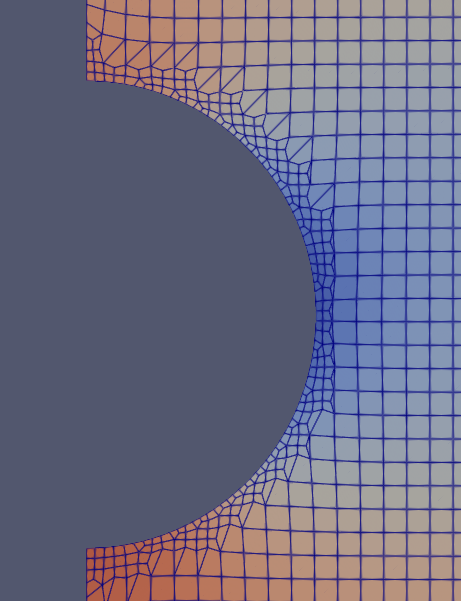
\includegraphics[height=1.85cm]{figures/equBall.png}\\[-0.04cm]
        {\tiny Start: nahezu kugelförmig}\\[0.12cm]
        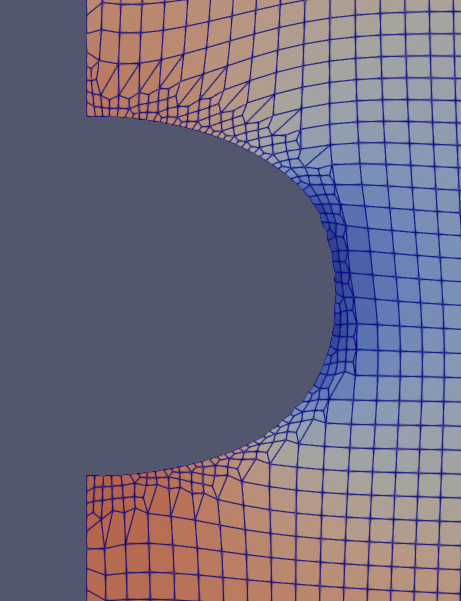
\includegraphics[height=1.85cm]{figures/equEllipsoid.png}\\[-0.04cm]
        {\tiny Ergebnis: abgeplatteter Ellipsoid}
    \end{center}
    \column{.66\linewidth}
    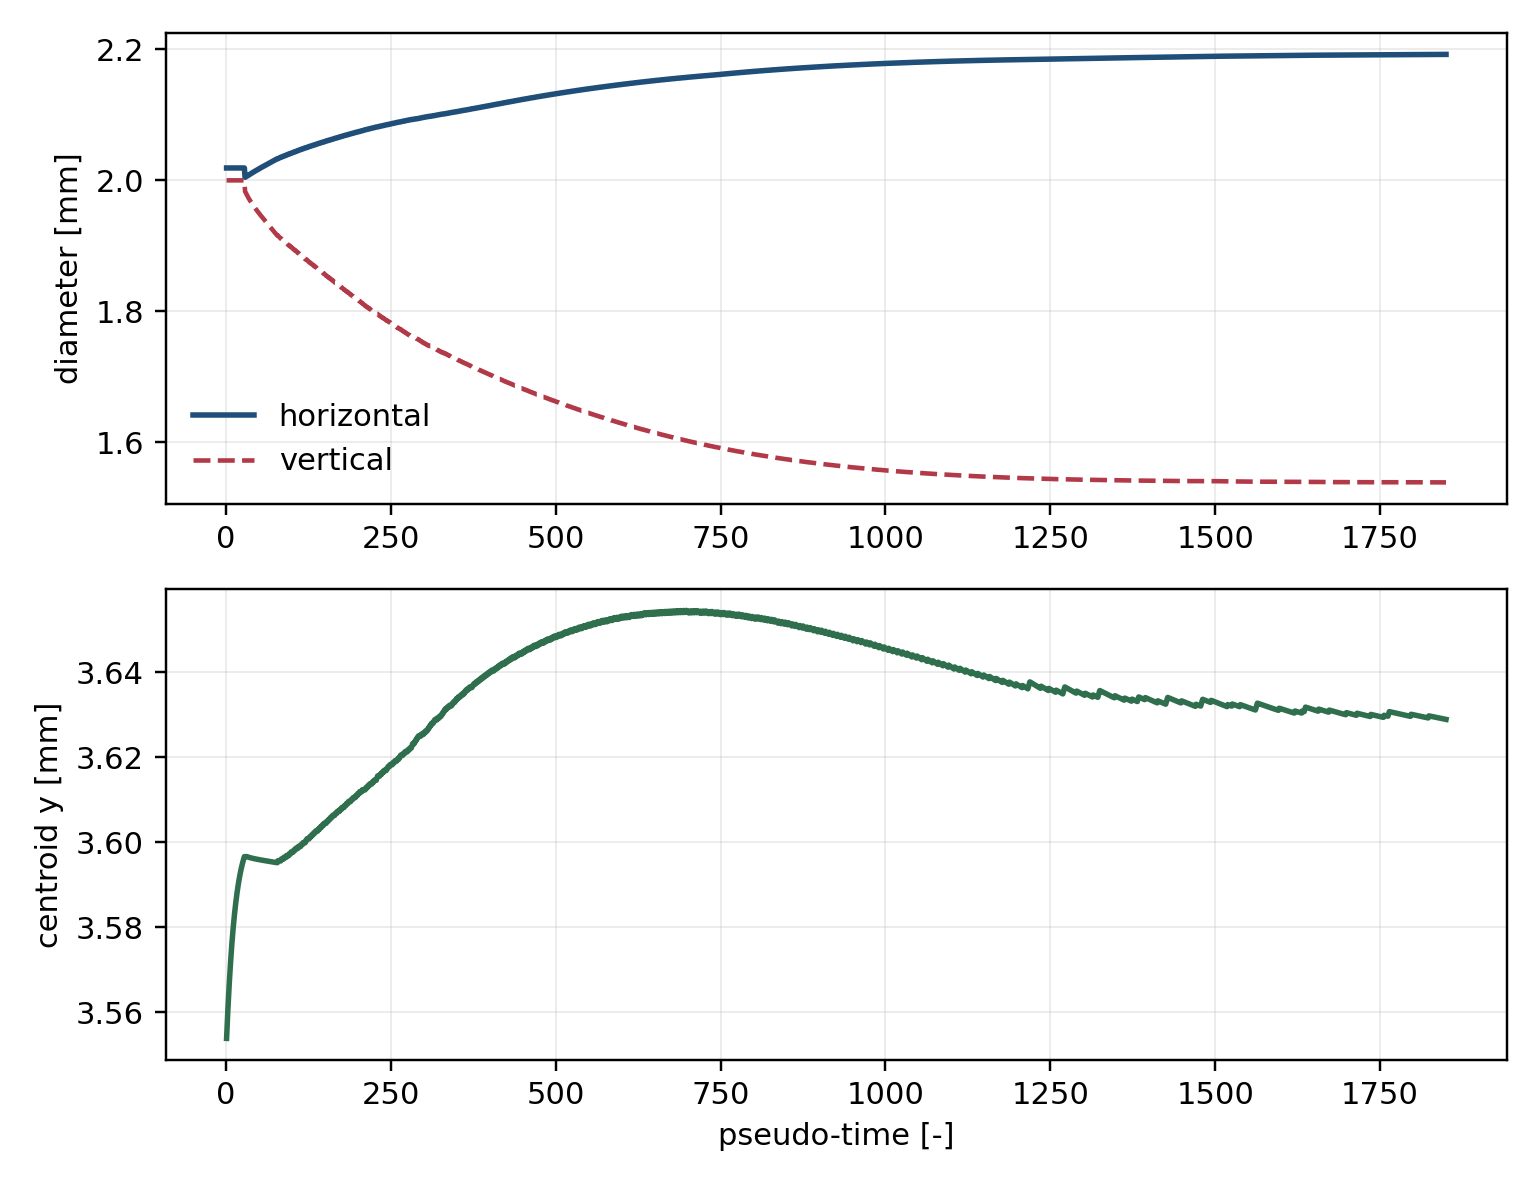
\includegraphics[height=4.15cm]{figures/shapePosition.png}
    \vspace{-0.1cm}
    {\scriptsize
    \begin{itemize}
        \setlength{\itemsep}{0.02cm}
        \item Der Pseudo-Solver trennt Positions- und Formkorrektur: zuerst wird $F_y\approx mg$ erreicht, danach wird die freie Oberfläche über das Young-Laplace-Residuum verschoben.
        \item Der horizontale Durchmesser wächst, der vertikale sinkt: der Tropfen wird ellipsoidisch abgeplattet.
        \item Die Schwerpunktlage nähert sich nach anfänglichem Überschwingen einem stabilen Bereich.
    \end{itemize}
    }
    \end{columns}
\end{frame}

\begin{frame}{Tensorielle PML: kleinere Dämpfungskoeffizienten}
    \begin{columns}
    \column{.55\linewidth}
    \begin{itemize}
        \item Der frühere isotrope Ansatz verwendet dieselbe Dämpfung in allen
        Raumrichtungen.
        \item Die tensorielle PML verwendet gerichtete Komponenten:
        \[
            \boldsymbol{\sigma}
            =(\sigma_x,\sigma_y,\sigma_z),
            \qquad
            \mathbf{T}_0,\mathbf{T}_1
            =\operatorname{diag}(T_{xx},T_{yy},T_{zz}).
        \]
        \item Nur die zur offenen Grenze normale Richtung wird gedämpft;
        tangentiale Richtungen bleiben unbeeinflusst.
        \item Damit reicht eine deutlich kleinere maximale Dämpfung für eine
        ausreichende Absorption.
    \end{itemize}
    \column{.45\linewidth}
    \begin{block}{Numerischer Vorteil}
        Sehr große Koeffizienten erzeugen einen steilen, vom Mesh schlecht
        aufgelösten Dämpfungsverlauf. Das kann numerische Reflexionen auslösen.
        Kleinere Koeffizienten reduzieren dieses Risiko deutlich.
    \end{block}
    \end{columns}
\end{frame}

\begin{frame}{Tensorielle PML: Verifikation}
    \begin{columns}
    \column{.46\linewidth}
    \begin{itemize}
        \item Verifikation am eindimensionalen Schichtfall mit analytischer Lösung.
        \item Mit
        \[
            |\sigma_{\max}|=2\times10^5\,\mathrm{s}^{-1}
        \]
        wird bereits eine relative Amplitudenabweichung von etwa
        $9.1\times10^{-4}$ erreicht.
        \item Eine weitere Erhöhung auf
        $5\times10^5\,\mathrm{s}^{-1}$ verbessert das Ergebnis praktisch nicht.
        \item Schlussfolgerung: ausreichende Dämpfung ohne unnötig große
        Koeffizienten und mit geringerem Reflexionsrisiko.
    \end{itemize}
    \column{.54\linewidth}
    \begin{center}
        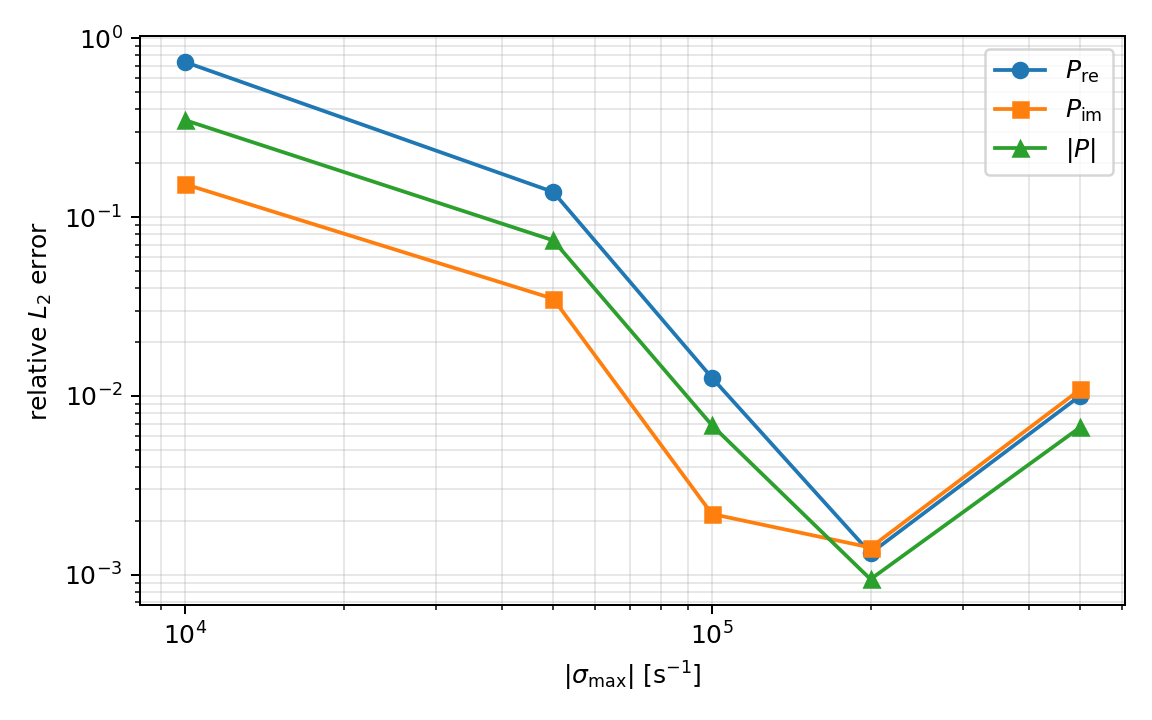
\includegraphics[width=\linewidth]{../paper_aHF/figures/pml_sigma_sensitivity.png}

        \vspace{0.1cm}
        \scriptsize Relative Fehler in der physikalischen Domäne für verschiedene PML-Dämpfungen.
    \end{center}
    \end{columns}
\end{frame}

\begin{frame}{Zusammenfassung des Fortschritts}
    \begin{enumerate}
        \item \textbf{Axisymmetrisches, lokal verfeinertes cfMesh-Mesh}
        \begin{itemize}
            \item ermöglicht die Gor'kov-Verifikation,
            \item ermöglicht mit \code{acousticDropEquilibriumFoam} die Suche
            nach Gleichgewichtsposition und -form.
        \end{itemize}
        \item \textbf{Tensorielle PML}
        \begin{itemize}
            \item erreicht ausreichende Absorption mit kleineren Koeffizienten,
            \item reduziert die Wahrscheinlichkeit numerischer Reflexionen.
        \end{itemize}
        \item \textbf{Forschungsstand}
        \begin{itemize}
            \item Ein ausgereiftes Werkzeug zur Untersuchung der
            Tropfendynamik im einachsigen Levitator.
            \item Als nächste Forschungsstufe im Zukunft kann der durch akustische
            Strömung induzierte Stofftransport an der Grenzfläche eines
            Tropfens im Gleichgewicht untersucht werden.
        \end{itemize}
    \end{enumerate}
\end{frame}

\begin{frame}{Rechenzeit reduzieren}
    \begin{itemize}
        \item Die wichtigste Herausforderung auf der numerischen Seite ist
        weiterhin die hohe Rechenzeit der gekoppelten Simulationen.
        \item Bereits untersuchte Optimierungsansätze:
        \begin{enumerate}
            \item lokale Mesh-Verfeinerung,
            \item adaptive Mesh-Verfeinerung (AMR),
            \item Wiederverwendung des akustischen Feldes über mehrere
            Strömungszeitschritte.
        \end{enumerate}
        \item HPCToolkit ist eingerichtet und ermöglicht eine systematische
        Analyse von Laufzeit, Skalierung und relevanten Hotspots.
        \item Bisher liefert keiner der untersuchten Ansätze eine
        zufriedenstellende und gleichzeitig robuste Leistungsverbesserung.
        \item Nächster Schritt: zunächst die dominanten Kosten mit HPCToolkit
        quantifizieren und anschließend gezielt Solver, Parallelisierung und
        Aktualisierungsstrategie optimieren.
    \end{itemize}
\end{frame}

\begin{frame}{Experimentplan zur Validierung}
    \begin{enumerate}
        \item \textbf{Strahlungskraft auf den Reflektor}
        \begin{itemize}
            \item Akustische Strahlungskraft für verschiedene Levitatorhöhen messen.
            \item Direkter und robuster Ausgangspunkt für den Vergleich des
            akustischen Feldes mit der Simulation.
        \end{itemize}
        \item \textbf{Frei levitierter Tropfen}
        \begin{itemize}
            \item Tropfenbewegung und -form mit einer Kamera aufzeichnen.
            \item Durch Bildverarbeitung Schwingungsfrequenz, Schwingungsamplitude
            und Gleichgewichts-Aspektverhältnis bestimmen.
            \item Geeignet für eine erste Validierung der gekoppelten Simulation.
        \end{itemize}
        \item \textbf{Am Reflektor haftender Tropfen}
        \begin{itemize}
            \item Schwaches Schallfeld anwenden: Der Tropfen deformiert sich,
            wird jedoch nicht levitiert.
            \item Definierte Position und Randbedingungen ermöglichen einen
            zuverlässigen Eins-zu-eins-Vergleich zwischen Experiment und Simulation.
        \end{itemize}
    \end{enumerate}
\end{frame}

\section{090726}
\begin{frame}{Numerische Dämpfung im 1D-Wellentest}
    \scriptsize
    \setlength{\abovedisplayskip}{0.04cm}
    \setlength{\belowdisplayskip}{0.04cm}
    \begin{columns}[T]
    \column{.52\linewidth}
    \begin{block}{Beobachtung}
        Im Fall \code{layeredInterface1D} nimmt die Amplitude auch dann mit der
        Ausbreitungsstrecke ab, wenn PML und Wasserphase entfernt sind.
    \end{block}
    \begin{itemize}
        \setlength{\itemsep}{0.05cm}
        \item Aktive Druckgleichung in \code{acousticWaveFoam}:
        \[
            \frac{1}{c_g^2}\frac{\partial^2 p}{\partial t^2}
            - \nabla^2 p = 0 .
        \]
        \item \code{d2dt2Schemes} = \code{Euler}; der Laplace-Term wird
        implizit am neuen Zeitschritt gelöst.
    \end{itemize}

    \column{.48\linewidth}
    \begin{block}{Diskreter Verstärkungsfaktor}
        Für eine Fourier-Mode ergibt sich näherungsweise
        \[
            \begin{aligned}
                \delta_{tt}p/c_g^2+k_h^2p^{n+1}&=0,\\
                |G|&=\frac{1}{\sqrt{1+(c_g\Delta t k_h)^2}}<1 .
            \end{aligned}
        \]
    \end{block}
    \begin{itemize}
        \setlength{\itemsep}{0.05cm}
        \item Für $f=20\,\mathrm{kHz}$ und $\Delta t=10^{-6}\,\mathrm{s}$:
        $|G|\approx0.992$ pro Zeitschritt.
        \item Über eine Periode: ca. $0.68$ der Anfangsamplitude.
        \item Hauptursache: numerische, nicht physikalische Dämpfung.
    \end{itemize}
    \end{columns}

    \vspace{-0.02cm}
    \begin{block}{Konsequenz}
        Kleinere Zeitschritte reduzieren die Dämpfung; für einen verlustfreien
        Testfall ist eine zentrierte, energieerhaltende Zeitintegration nötig.
        Das rechte \code{zeroGradient}-Ende kann zusätzlich Reflexionen erzeugen.
    \end{block}
\end{frame}

\begin{frame}{Berechnung des Verstärkungsfaktors}
    \scriptsize
    \setlength{\abovedisplayskip}{0.05cm}
    \setlength{\belowdisplayskip}{0.05cm}
    \begin{columns}[T]
    \column{.50\linewidth}
    \begin{block}{Diskrete Mode}
        Für eine räumliche Eigenmode gilt
        \[
            -\nabla_h^2\phi = \lambda_h\phi ,
        \]
        und die implizite Zeitschrittgleichung wird zu
        \[
            \frac{p^{n+1}-2p^n+p^{n-1}}{c_g^2\Delta t^2}
            +\lambda_h p^{n+1}=0 .
        \]
    \end{block}
    \begin{itemize}
        \setlength{\itemsep}{0.04cm}
        \item Ansatz: $p^n=G^n p^0$.
        \item $G$ beschreibt die Änderung der Amplitude pro Zeitschritt.
    \end{itemize}

    \column{.50\linewidth}
    \begin{block}{Quadratische Gleichung}
        Einsetzen und Kürzen liefert
        \[
            \frac{G^2-2G+1}{c_g^2\Delta t^2}
            +\lambda_h G^2=0 .
        \]
        Mit $\mu^2=c_g^2\Delta t^2\lambda_h$:
        \[
            (1+\mu^2)G^2-2G+1=0 .
        \]
    \end{block}
    \begin{itemize}
        \setlength{\itemsep}{0.04cm}
        \item Lösung:
        \[
            G=\frac{1\pm i\mu}{1+\mu^2},
            \qquad
            |G|=\frac{1}{\sqrt{1+\mu^2}} .
        \]
        \item Weil $|G|<1$, wird jede Mode numerisch gedämpft.
    \end{itemize}
    \end{columns}
\end{frame}

\begin{frame}{Abschätzung für den 20-kHz-Testfall}
    \scriptsize
    \setlength{\abovedisplayskip}{0.05cm}
    \setlength{\belowdisplayskip}{0.05cm}
    Für eine schwach gedämpfte laufende Welle kann $\lambda_h\approx k^2$ mit
    $k=\omega/c_g$ gesetzt werden. Damit folgt
    \[
        \mu=c_g\Delta t k=\omega\Delta t=2\pi f\Delta t .
    \]

    \begin{block}{Aktuelle Parameter}
        \[
            f=20\,\mathrm{kHz},
            \qquad
            \Delta t=10^{-6}\,\mathrm{s},
            \qquad
            \mu=2\pi\cdot 20000\cdot10^{-6}\approx0.1257 .
        \]
        \[
            |G|=\frac{1}{\sqrt{1+0.1257^2}}\approx0.9922 .
        \]
    \end{block}

    \begin{itemize}
        \setlength{\itemsep}{0.05cm}
        \item Ein Zeitschritt erhält ca. $99.22\,\%$ der Modenamplitude.
        \item Eine Periode besitzt $1/(f\Delta t)=50$ Zeitschritte.
        \item Daher:
        \[
            |G|^{50}\approx 0.9922^{50}\approx0.68 .
        \]
        \item Diese Dämpfung entsteht aus der Diskretisierung, nicht aus PML,
        Wasserphase oder physikalischer Viskosität.
    \end{itemize}
\end{frame}

\begin{frame}{Lösung: zentrierte Laplace-Diskretisierung}
    \scriptsize
    \setlength{\abovedisplayskip}{0.04cm}
    \setlength{\belowdisplayskip}{0.04cm}
    \begin{columns}[T]
    \column{.48\linewidth}
    \begin{block}{Ursprüngliches Problem}
        Die voll implizite Form
        \[
            \delta_{tt}p/c^2-\nabla_h^2p^{n+1}=0
        \]
        ist stabil, aber nicht amplitudenerhaltend:
        \[
            |G|=\frac{1}{\sqrt{1+\mu^2}}<1 .
        \]
    \end{block}
    \begin{itemize}
        \setlength{\itemsep}{0.04cm}
        \item Die Dämpfung entsteht nicht durch PML, sondern durch den
        neuen Zeitlevel im Laplace-Term.
        \item Nur $\Delta t$ zu verkleinern reduziert den Fehler, beseitigt ihn
        aber nicht grundsätzlich.
    \end{itemize}

    \column{.52\linewidth}
    \begin{block}{Eingesetzte Form}
        \[
            \delta_{tt}p/c^2
            -\nabla_h^2\left(
                \frac{p^{n+1}+2p^n+p^{n-1}}{4}
            \right)=0 .
        \]
        Im Code:
        \[
            -\frac14 L(p^{n+1})
            -\frac12 L(p^n)
            -\frac14 L(p^{n-1}) .
        \]
    \end{block}
    \begin{itemize}
        \setlength{\itemsep}{0.04cm}
        \item Das ist eine trapez-/Newmark-artige Zentrierung.
        \item Für verlustfreie Fourier-Moden gilt $|G|=1$:
        Phasenfehler bleibt möglich, künstliche Amplitudendämpfung nicht.
    \end{itemize}
    \end{columns}
\end{frame}

\begin{frame}{Umsetzung in \code{acousticWaveFoam}}
    \scriptsize
    \setlength{\abovedisplayskip}{0.04cm}
    \setlength{\belowdisplayskip}{0.04cm}
    \begin{block}{Aktuelle Druckgleichung mit Medienfaktoren}
        \[
        \begin{aligned}
            &\partial_{tt}\left(\frac{c^{-2}}{\rho}p\right)
            -\frac14\nabla_h\cdot\left(\rho_f^{-1}\nabla_h p^{n+1}\right)\\
            &\quad
            -\frac12\nabla_h\cdot\left(\rho_f^{-1}\nabla_h p^n\right)
            -\frac14\nabla_h\cdot\left(\rho_f^{-1}\nabla_h p^{n-1}\right)
            +\text{PML-Terme}=0 .
        \end{aligned}
        \]
    \end{block}

    \begin{columns}[T]
    \column{.52\linewidth}
    \begin{itemize}
        \setlength{\itemsep}{0.05cm}
        \item \code{invc2/rho} bleibt im Trägheitsterm erhalten.
        \item \code{invRhof} bleibt im Flussterm erhalten.
        \item Die implizite Matrix enthält nur den Anteil bei $p^{n+1}$;
        die Anteile bei $p^n$ und $p^{n-1}$ stehen explizit auf der rechten Seite.
    \end{itemize}

    \column{.48\linewidth}
    \begin{block}{Warum genau so?}
        Diese Form erhält die symmetrische Kopplung zwischen Druckträgheit und
        akustischem Fluss, vermeidet aber die rein numerische Dämpfung der
        voll impliziten Laplace-Auswertung.
    \end{block}
    \begin{itemize}
        \setlength{\itemsep}{0.05cm}
        \item PML-Dämpfung bleibt absichtlich erhalten.
        \item In der physikalischen Domäne muss \code{SC0}, \code{SC1},
        \code{SC2} verschwinden.
    \end{itemize}
    \end{columns}
\end{frame}

\begin{frame}{Korrektur des 1D-Testfalls}
    \scriptsize
    \setlength{\abovedisplayskip}{0.04cm}
    \setlength{\belowdisplayskip}{0.04cm}
    \begin{columns}[T]
    \column{.50\linewidth}
    \begin{block}{Warum der Rand geändert wurde}
        Nach Entfernen der numerischen Dämpfung wurde die frühere
        \code{uniformFixedGradient}-Anregung sehr empfindlich: sie erzwingt
        eine Neumann-Bedingung an einem endlichen, reflektierenden 1D-Kanal.
    \end{block}
    \begin{itemize}
        \setlength{\itemsep}{0.05cm}
        \item Das ist für einen Piston physikalisch interpretierbar.
        \item Für einen reinen Propagationstest vermischt es jedoch
        Anregung, Reflexion und numerische Eigenschaften.
    \end{itemize}

    \column{.50\linewidth}
    \begin{block}{Neuer Test-Rand}
        Für den Diagnosefall wird der erwartete Druck direkt vorgegeben:
        \[
            p_\mathrm{amp}=\rho_g c_g U_\mathrm{piston}.
        \]
        Mit den aktuellen Werten:
        \[
            p_\mathrm{amp}=1.2\cdot343\cdot0.01
            \approx4.116\,\mathrm{Pa}.
        \]
    \end{block}
    \begin{itemize}
        \setlength{\itemsep}{0.05cm}
        \item \code{uniformFixedValue sine}
        \item Amplitudenvergleich misst nun die Propagation, nicht die
        Piston-Neumann-Kopplung.
    \end{itemize}
    \end{columns}
\end{frame}

\begin{frame}{Verifikation nach der Korrektur}
    \scriptsize
    \setlength{\abovedisplayskip}{0.04cm}
    \setlength{\belowdisplayskip}{0.04cm}
    \begin{block}{Test}
        \code{layeredInterface1D}, ohne Wasserphase und ohne PML-Dicke:
        $L=0$, $\alpha_\mathrm{water}=0$, $f=20\,\mathrm{kHz}$,
        $\Delta t=10^{-6}\,\mathrm{s}$.
    \end{block}

    \begin{center}
    \begin{tabular}{cc}
        \toprule
        Probe $x$ [m] & Max. Amplitude nach Ankunft [Pa]\\
        \midrule
        0.05 & 4.10\\
        0.08 & 4.12\\
        0.10 & 4.11\\
        0.14 & 4.11\\
        0.22 & 4.15\\
        \bottomrule
    \end{tabular}
    \end{center}

    \begin{itemize}
        \setlength{\itemsep}{0.05cm}
        \item Erwartete Amplitude: $4.116\,\mathrm{Pa}$.
        \item Relative Streuung über alle Proben: ca. $1.2\,\%$.
        \item Ergebnis: die vorherige distanzabhängige Dämpfung ist entfernt;
        verbleibende Unterschiede kommen aus Transienten, Randreflexionen und
        Diskretisierungsfehlern.
    \end{itemize}
\end{frame}

\bibliographystyle{plainnat} % Choose an appropriate style
\bibliography{bibliography}
\end{document}
